\documentclass[a4paper,class=article,border=10pt,tikz]{standalone}

%mypackages
\usepackage{pythontex}
\usepackage{pgfplots}
\usepackage{amsmath}
\usepackage{titlesec}
\usepackage{tikz}
\usetikzlibrary{shapes.geometric}
\usetikzlibrary{positioning}
\usetikzlibrary{snakes,calc,positioning,patterns,angles,quotes,decorations.pathmorphing,decorations.markings}
% \titleformat{<command>}[<shape>]{<format>}{<label>}{<sep>}{<before-code>}[<after-code>]
%\titleformat{\section}{\normalfont\Large\bfseries}{\thesection.}{10pt}{}
% \titlespacing{<command>}{<left>}{<before-sep>}{<after-sep>}
%\titlespacing{\section}{0pt}{14pt}{7pt}

%\titleformat{\subsection}{\normalfont\itshape}{\thesubsection.}{10pt}{}
%\titlespacing{\subsection}{0pt}{12pt}{6pt}
% set font encoding for PDFLaTeX, XeLaTeX, or LuaTeX
\usepackage{ifxetex,ifluatex}
\if\ifxetex T\else\ifluatex T\else F\fi\fi T%
  \usepackage{fontspec}
\else
  \usepackage[T1]{fontenc}
  \usepackage[utf8]{inputenc}
  \usepackage{lmodern}
\fi

\usepackage{hyperref}


\title{Title of Document}
\author{Name of Author}

% Enable SageTeX to run SageMath code right inside this LaTeX file.
% http://doc.sagemath.org/html/en/tutorial/sagetex.html
% \usepackage{sagetex}

% Enable PythonTeX to run Python – https://ctan.org/pkg/pythontex
% \usepackage{pythontex}

\begin{document}

% parametric pendulum + sway czy tam surge

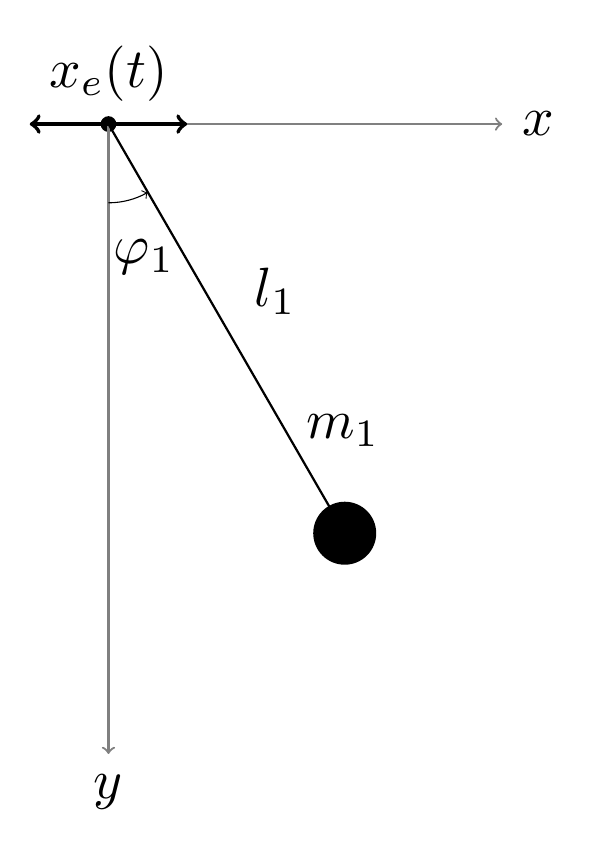
\begin{tikzpicture}[scale=2, every node/.style={scale=2}]
 \coordinate (origo) at (0,0);
 \coordinate (pivot) at (1,5);

    % draw axes
    \fill[black] (origo) circle (0.05);
    \draw[thick,gray,->] (origo) -- ++(2.5,0) node[black,right] {$x$};
    \draw[thick,gray,->] (origo) -- ++(0,-4) node (mary) [black,below] {$y$};
    \draw[<->,line width=1.5pt] (-0.5,0)--(0.5,0) node[midway,above]{$x_{e}(t)$};

    % draw roof
    %\fill[pattern = north east lines] ($ (origo) + (-1,0) $) rectangle ($ (origo) + (1,0.3) $);
    %\draw[thick] ($ (origo) + (-1,0) $) -- ($ (origo) + (1,0) $);

    \draw[thick] (origo) -- ++(300:3) coordinate (bob1) node[near end, right]{$m_{1}$};
    \node (l1_label) at ($(origo)+(315:1.5cm)$)   {$l_{1}$};
    \fill (bob1) circle (0.2);

    \pic [draw, ->, "$\varphi_{1}$", angle eccentricity=1.75] {angle = mary--origo--bob1};
\end{tikzpicture}
\end{document}
